\documentclass[10pt,a4paper]{article}
\usepackage[utf8]{inputenc}
\renewcommand{\familydefault}{\sfdefault}
\usepackage{amsmath,amssymb,sansmathfonts,color,graphicx,afterpage,mathtools,bm,hyperref,listings,subcaption}
\graphicspath{{figures/}}
\usepackage[margin=2cm]{geometry}
\usepackage{cancel}
\setlength{\parskip}{3pt}
\allowdisplaybreaks
\lstset{language=C++, basicstyle=\ttfamily}
\mathtoolsset{showonlyrefs}

\title{\textbf{Control Theory -- Assignments}}
\date{\vspace{-5ex}}

% % show solution?
% \newif\ifsolution
% %\solutiontrue
% \solutionfalse
%
% \newcommand{\sol}[1]{\noindent \textcolor{blue}{\ifsolution \emph{#1} \fi}}%

\begin{document}

\maketitle

\section{Introduction}
The evaluation of the course Control Theory is based on practical assignments in which you will apply several techniques taught during the course in order to control the cart presented in Figure \ref{fig:cart}. All carts have two separately driven wheels in the front. At the back, one type of cart is equipped with a free axle with two wheels, for moving on a straight line, while the other carts have a swivel wheel to allow rotation. The carts are controlled by an Arduino Mega, running MicroOS as software framework. For more information on this system, you are referred to the tutorial session.

You work in groups of 2 students. Be sure to \textbf{register your team by Sunday October 21, 2018} in the provided \href{https://tolapps.kuleuven.be/Tolinto/event/9350079486_gII}{Tolinto module}. After the registration, you will get a cart assigned to you, which you will need to share with one other team. If your cart has a swivel wheel, you must perform assignments 1, 2, 3 and 5. Students with a 4-wheeled cart perform assignments 1, 2, 3 and 4. If for some reason you are alone in a group (e.g. your team partner stopped following the course), you still perform the assignments as a group of 2 students.

\begin{figure}[h]
  \centering
  \begin{subfigure}[c]{0.46\columnwidth}
    \centering
    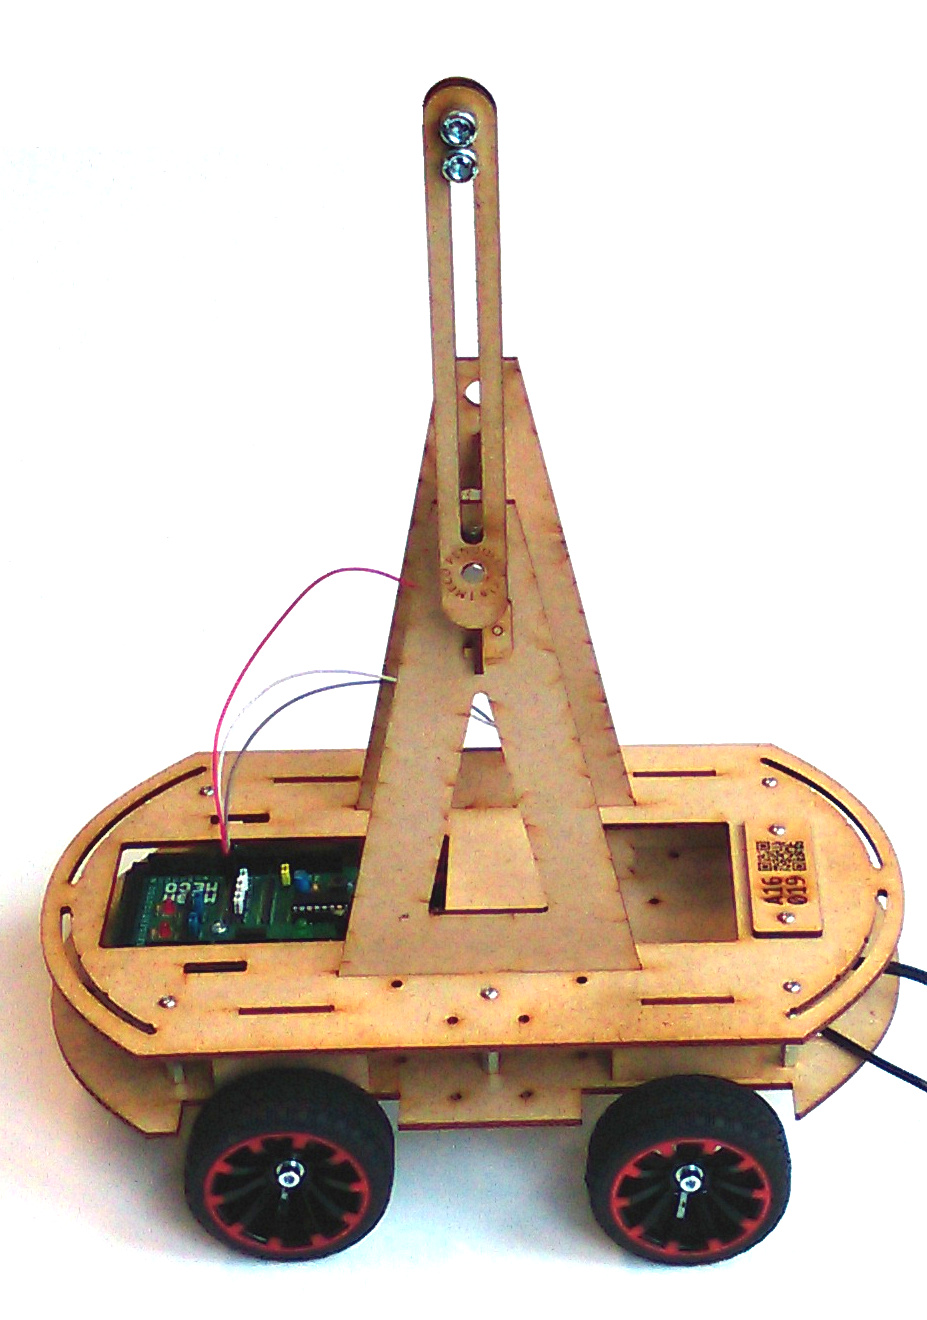
\includegraphics[scale=0.1]{figures/pendulum.jpg}
    \caption{4-wheeled cart with pendulum}
  \end{subfigure}
  \begin{subfigure}[c]{0.46\columnwidth}
    \centering
    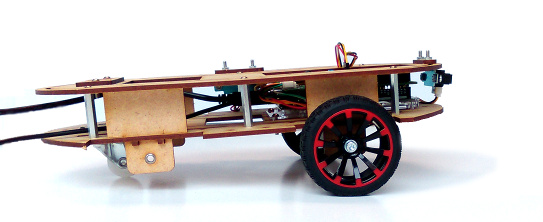
\includegraphics[scale=0.4]{figures/swivel.jpg}
    \caption{Cart with swivel wheel}
  \end{subfigure}
\caption{Setup used during the assignments.}
\label{fig:cart}
\end{figure}

\subsection{Instructions for the evaluation}
You write your answers to the assignments down in a slideshow that is understandable on its own. In addition, we ask for the source codes of your implementations as well as a movie of one of your experiments. In a second step, you will be invited to defend your work orally.

The \textbf{deadline} for handing in your presentation plus source files and movie, as well as for registering your team for a time slot for the oral defense is \textbf{Friday December 21, 2018}. At that time a submission module will be made available on Toledo, in the menu ``Assignments'', for uploading the required files; and a Tolinto subscription module will be launched for the oral defense registration.

Please read the following instructions carefully and comply with them!

\subsubsection*{Instructions for the presentation}
	\begin{itemize}
	\item On the title slide, clearly mention your team number (as mentioned in the teams-carts assignments list on Toledo), your platform ID, and your names.
  \item Answer all questions of the assignments. All questions are assessed.
  \item Provide answers in a clear way. Bullet lists are preferred over full text. However, try to be complete.
  \item Provide clear figures: all lines and colors must be visible, and axes must have readable labels with physical units.
  \item Slides should reflect the assignments: stick to the titles and divisions as mentioned in the assignment.
	\item The slides may be in English or in Dutch, as you prefer.
	\item Save the presentation in pdf format: \verb"teamXX_2018_presentation.pdf", with XX your team number. Make sure to number your slides. This facilitates the walk through your results at the oral defense.
	\end{itemize}


\subsubsection*{Instructions for the movie}
	\begin{itemize}
	\item Film your most advanced successful experiments with a camera, tablet, or smartphone. If you have no such device, contact the teaching team to borrow a camera.
	\item Make sure the platform ID as well as one of the team members' student card is clearly visible in the movie.
	\item Make sure your movie is compressed (web-optimized). Software suggestion: \href{https://handbrake.fr/}{HandBrake}.
	\item Save in MP4 format: \verb"teamXX_2018_movie.mp4", with XX your team number.
	\end{itemize}

\subsubsection*{Instructions for the source code}
	\begin{itemize}
	\item Compress your Matlab files as well as the entire Arduino sketchbook folder into one zip file: \verb"teamXX_2018_source.zip", with XX your team number.
	\item Make sure the code is stand-alone executable (include all ``helper'' files), and to select logical names for the main routines.
	\end{itemize}

\subsubsection*{Instructions for the oral defense}
\begin{itemize}
\item The oral defense comprises 20 minutes of questioning by the examiners. You may expect
		\begin{itemize}
		\item questions on the project and the approach taken in the assignments;
		\item questions on the course material to probe deeper insight and understanding.
		\end{itemize}
\item Bring your own laptop, on which you can show
		\begin{itemize}
		\item the presentation as submitted on Toledo;
		\item the movie submitted on Toledo.
		\end{itemize}
\item The defense will be in English or in Dutch, according to your preference.
\end{itemize}


\subsection{Support and feedback sessions}
In case there are questions, we strongly encourage you to consult with your fellow students. Discuss your findings and questions amongst yourselves and try to come up with an explanation or an answer. A dedicated forum is also made available on Toledo for this purpose. In case you cannot get to a consensus, you can ask the teaching assistants to help you out. They will be available for questions \textbf{during plenary feedback sessions only}:
\begin{itemize}
\item \textbf{assignment 1} (identification): Friday November 9, 4-6 PM, Aud. D
\item \textbf{assignment 2} (velocity control): Friday November 30, 4-6 PM, Aud. B
\item \textbf{assignment 3} (position control): Monday December 10, 4-6 PM, Aud. A
\item \textbf{assignment 4/5} (pendulum or trajectory tracking control): Friday December 14, 4-6 PM, Aud. B
\end{itemize}

In these sessions, only questions concerning one specific assignment will be treated. Therefore, make sure to keep on schedule with your assignments! Keep in mind, furthermore, that the assignments serve as your examination, so do not expect the assistants to solve them on your behalf.

In case your cart is broken, please don't hesitate to pass by the teaching assistants (rooms 01.17 and 01.19) as soon as possible such that we can fix whatever is broken. Do not put broken carts back in the cupboard without further notice!

\newpage
\section{Assignments}

If your cart has a swivel wheel, you must perform assignments 1, 2, 3 and 5. Students with a 4-wheeled cart perform assignments 1, 2, 3 and 4.

\subsection{Assignment 1: identification of the motors}
\begin{enumerate}
  \item Derive a theoretical model of a DC motor.
  \begin{enumerate}
    \item Write down the continuous-time transfer function from motor voltage to rotational velocity.
    \item What are the inputs, outputs and states? And what are their physical units?
    \item What assumptions and simplifications do you make?
    \item Discretize the system using a backward Euler method. Write down the discrete-time transfer function.
  \end{enumerate}
  \item Identify each `DC motor plus wheel' unit by exciting the motor while holding the cart in the air.
  \begin{enumerate}
    \item Which excitation signal do you apply? Why?
    \item Do you use filtering to improve the identification? Why? Which filter do you choose, and how do you select its parameters? Which signals do you filter?
    \item How do you obtain your system parameters? Write down the recursion expression and criterion that you used to estimate the parameters.
    \item Validate your identified model experimentally and plot the difference in response of the simulated model and the real system. As any physical system, the 'DC motor plus wheel' is in practice nonlinear. Prove this experimentally by checking for violations of the superposition principle\footnote{$F(x+y)=F(x)+F(y),\,F(ax)=aF(x)$} that holds for linear systems.
  \end{enumerate}
  \item Identify the cart.
  \begin{enumerate}
    \item Place the cart on the ground and validate the identified models of the two DC motors again. Are there differences? Explain them.
    \item Identify the motors again with the cart placed on the ground. Are the model parameters different? If so, give a (qualitative) explanation for it.
  \end{enumerate}
\end{enumerate}

\subsection{Assignment 2: velocity control of the cart}
\begin{enumerate}
  \item Design for each DC motor a velocity controller that yields zero steady-state error on a constant velocity reference. Design the controller using frequency response methods. Use the identified models of Assignment 1.
  \begin{enumerate}
    \item What type of controller do you choose? Why?
    \item Explain the design process and all choices of design parameters (phase margin, cut-off frequency, integration time, ...)
    \item Is there a theoretical limitation on the closed-loop bandwidth that can be achieved? Is there a practical limitation?
    \item Illustrate the design process with appropriate Bode diagrams.
  \end{enumerate}
  \item Validate the designed controller experimentally.
  \begin{enumerate}
    \item Implement the controller for both wheels on the Arduino and apply a step input for the reference velocity. Plot the error between the reference and measured velocity, and plot the corresponding actuator signals.
		\item Compare the measured response to the simulated response by plotting them both in the same figure. Do this for the velocity as well as for the actuator signals.
    \item Find a way of applying a constant force disturbance to the cart. Is your controller still following the velocity setpoint? Why?
  \end{enumerate}
\end{enumerate}

\subsection{Assignment 3: state feedback and state estimation}
In this assignment you will control the position of the cart while driving on a straight line (i.e. both velocity controlled motors should get the same velocity setpoint $v$). To this end, a position control loop is added on top of the velocity controllers designed in assignment~2. For the position control you will design a state feedback controller. In order to retrieve an estimate of the state, you will implement a Kalman filter. This filter uses distance measurements from the frontal infrared sensor to correct its estimate. This infrared sensor measures the distance to a wall in front of the cart. The origin is chosen on the wall. As the cart is positioned at the negative side of the origin, the infrared sensor measures $-x$, which is a positive value. To model the cart, you can assume the velocity control loop is ideal, i.e. you assume that the desired velocity is equal to the real velocity of the cart.

\begin{figure}[h]
\centering
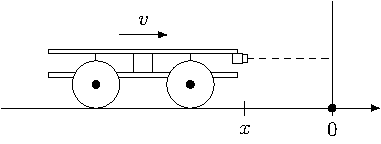
\includegraphics[scale=1]{figures/1dcart.pdf}
\caption{Cart measuring its distance to a wall.}
\end{figure}

For this assignment you can use the Arduino code provided on Toledo. This code implements a working Kalman filter and applies a reference velocity signal to the motors to actuate the cart. The implementation expects QRoboticsCenter to broadcast the input signal, the contents of a comma-separated values (CSV) file are sent to the cart line by line.\footnote{Details on reading CSV files in QRoboticsCenter can be found in the PDF of the tutorial sessions.} The CSV file \verb"csv/csv_linear_velocity_reference.txt" should be used to feed the reference signal for your cart velocity (in meters!) to the platform at a rate of 10\,Hz. You should extend the code by implementing the speed controller you designed in assignment~2. The comments in \verb"robot.cpp" provide the body of an implementation and guide you where to add calls to your speed control routines. For your convenience, the position controller is already implemented, you should however adapt the control gain $K$. Likewise, in the Kalman filter, the process noise covariance $Q$ and the measurement noise covariance $R$ need to be tuned, which can be found in \verb"kalman_filter.cpp". Throughout the assignment you can assume a constant $Q$ and $R$. With a working position controller in place a different CSV file must be used, namely \verb"csv/csv_position_reference.txt" (10\,Hz), which supplies the position reference (constant by default) and the corresponding velocity feedforward signals. If you want to test your Kalman filter and state feedback design for other motions, you can generate your own position reference through the file \verb"csv/csv_position_reference.m".

\begin{enumerate}
  \item State feedback controller design.
  \begin{enumerate}
    \item Write down the state equation in discrete form. The velocity of the cart can be seen as input. Use a forward Euler method as discretization scheme.
    \item Derive an expression for the pole of the closed-loop system as a function of the sample time $T_s$ and the state feedback gain $K$. What happens with the pole when you increase or decrease $K$? What happens with the closed-loop response? Can we choose $K$ such that the system becomes unstable?
  \end{enumerate}

  \item Kalman filter insight.
  \begin{enumerate}
    \item Write down the measurement equation.
    \item Derive an expression for the (time-varying) Kalman gain $L_{k+1}$ as a function of the state estimate covariance $\hat{P}_{k|k}$, the process noise covariance $Q$ and measurement noise covariance $R$. How does $L_{k+1}$ evolve when $Q\rightarrow\infty$? How does $L_{k+1}$ evolve when $R\rightarrow\infty$? Is this what you expect?
    \item Derive an expression for the next state estimate covariance $\hat{P}_{k+1|k+1}$ as a function of the previous state estimate covariance $\hat{P}_{k|k}$, the process noise covariance $Q$ and measurement noise covariance $R$. How does $\hat{P}_{k+1|k+1}$ evolve when $Q\rightarrow\infty$? How does $\hat{P}_{k+1|k+1}$ evolve when $R\rightarrow\infty$? Is this what you expect?
    \item Derive an expression for the steady-state covariance $\hat{P}_\infty$ and related Kalman gain $L_\infty$ as a function of $Q$ and $R$. This gain should be equal to gain of a Linear Quadratic Estimator. Check this for some numerical value for $Q$ and $R$ using the \texttt{dlqr} command in Matlab.
    \item Derive an expression for the closed-loop pole of the Linear Quadratic Estimator as a function of $\frac{Q}{R}$. What happens with the pole when you increase or decrease $\frac{Q}{R}$. Is this what you expect? Can we choose $\frac{Q}{R}$ such that the system becomes unstable?
  \end{enumerate}
\newpage
  \item State feedback and state estimator implementation.
  \begin{enumerate}
    \item Choose appropriate values for the control gain $K$, process noise covariance $Q$ (see the \texttt{TimeUpdate}-routine in \texttt{kalman\_filter.cpp}) and measurement noise covariance $R$ (\texttt{MeasurementUpdate}-routine in \texttt{kalman\_filter.cpp}). Adapt these values in the C++ code provided on Toledo. Also, make sure to set the initial state estimate and its covariance appropriately in the \texttt{resetKalmanFilter}-routine in \texttt{robot.cpp}.\\
    For the sub-assignments below, a step response can be generated by applying a constant position reference that differs from the cart's initial position to the position control loop. You can adjust this reference in the Matlab script (\texttt{csv\_position\_reference.m}), which creates the corresponding CSV-file \verb"csv/csv_position_reference.txt".

		%let QRoboticsCenter send the contents of a CSV-file as a reference position and feed-forward velocity. A step reference is generated by entering a constant position reference in the Matlab script (\texttt{csv\_position\_reference.m}) creating the CSV-file. Make sure to modify the initial state estimate and its covariance according to the task by modifying them in the \texttt{void Robot::resetKalmanFilter}-routine in \texttt{robot.cpp}.  Why are the velocity feed-forwards in the tasks below always zero? Analyze the CSV-file, what is the reference position, where will you place the cart initially?}
    \item Apply a step-signal as position reference for different values of $K$. Illustrate the different step responses in one plot, and do the same for the corresponding control signals. Explain the plots using the analysis made in 1b.
    \item Apply a step-signal as position reference for different values of $\frac{Q}{R}$ (e.g., values between $10^{-4}$ and $1$). Plot the evolution of $\hat{P}_{k|k}$ in one plot and the evolution of $L_{k}$ in another plot. Explain the plots using the analysis of 2e. Do the values converge towards respectively $\hat{P}_\infty$ and $L_\infty$, computed in 2d?
    \item Using the data from the previous question (3c), calculate the evolution of the NIS and the SNIS, and check whether their values are within a certain confidence interval (e.g. 95\%) for the distribution you would expect. Is your Kalman filter consistent? If not, can you think of possible causes for this?
    \item Use a wrong initial estimation for the position. Apply a step in desired position. Plot the evolution of the position estimate together with the measured position by the infrared sensor. Do this for different values of $\frac{Q}{R}$. Explain the different responses.
    \item Choose the estimator gain now such that the closed-loop pole of the estimator is 10x \emph{slower} than the closed-loop pole of the controller. Start from an initial estimation error. Apply a step in desired position. Plot the estimated position and measured position in one plot. Explain the observed behavior.
  \end{enumerate}
\end{enumerate}

\subsection{Assignment 4: control of a pendulum}
This assignment uses a cart with a pendulum. The pendulum is attached to a rotary potentiometer which allows you to measure the pendulum angle. In this assignment you will design a state feedback controller to control the position of the pendulum mass. A state estimator will be required for providing the controller with state information. In this assignment you can again assume that the velocity control loop is ideal. You should only concentrate on the pendulum in its stable position.

\begin{enumerate}
  \item Model and identify the system.
  \begin{enumerate}
    \item Derive a theoretical continuous model of the velocity-steered cart with a pendulum.
    \item Derive a state-space equation for the nonlinear model (i.e. $\dot{\xi}=f(\xi, v)$). Use as states $\xi=[x, \theta, l\dot{\theta}+\dot{x}\cos\theta]^T$, with $x$ the position of the cart and $\theta$ the pendulum angle.
    \item Linearize the model around the pendulum's stable point. Write down the state space description and corresponding transfer function.
    \item Apart from the gravitational constant $g=9.81$ m/s, the pendulum length and damping coefficient are the only parameter in the model. Measure the length with a ruler. This length could also be derived from the pendulum's natural frequency. Perform an experiment from which you can deduce the natural frequency and therefore the pendulum length. Can you also derive the damping ratio and therefore the damping coefficient? Illustrate this experiment with a figure illustrating your measurements. Describe how you computed the required system parameters. In the remainder of this assignment, you may neglect the damping in the system.
    \item Discretize the linear and nonlinear system using a forward Euler method. In the remainder we focus on these descretized versions.
  \end{enumerate}
    \item Design and implement a linear Kalman filter.
  \begin{enumerate}
    \item Design a linear Kalman filter based on the linearized system equations. Use the encoders as position measurement and the potentiometer as angle measurement. Implement the steps on the Arduino. Apply a hat-function as input velocity. Monitor the evolution of the estimation error covariance $\hat{P}_{k|k}$ and Kalman gain $L_k$ for different values of $\frac{Q}{R}$. Explain what happens when decreasing/increasing $\frac{Q}{R}$.
  \end{enumerate}
  \item Design and implement an extended Kalman filter.
    \begin{enumerate}
    \item Design an extended Kalman filter based on the nonlinear system equation. Write down the state equation and measurement equation.
  \item Write down the Jacobian of the state and measurement equation.
  \item Implement the extended Kalman filter on the Arduino. Compare its convergence with the linear Kalman filter.
  \end{enumerate}
  \item Design and implement a state feedback controller based on the linearized model.
  \begin{enumerate}
    \item Design a Linear Quadratic Regulator that makes a trade-off between penalizing deviations in the pendulum's mass position and actuation effort. Clearly indicate the objective that the LQR is minimizing.
    \item Design a feedforward gain such that zero steady-state errors occur for a step reference in desired pendulum mass position.
    \item Implement the controller on the Arduino using your Kalman estimator. Apply a step in the reference for the pendulum mass position. Visualize in one plot the responses for different trade-offs between reference tracking and actuation effort. Plot the actuator signal as well.
  \end{enumerate}
\end{enumerate}

\subsection{Assignment 5: estimation and control of a two-wheel driven cart}
This assignment considers the cart mounted with the swivel wheel and with two infrared sensors. Because the cart has two separately driven wheels, it acts as a two-wheel drive (2WD) system that can move in the horizontal plane.
The system under consideration is shown in Figure \ref{fig:cartkalman}. The 2WD cart moves around in the world's $XY$ plane. The coordinates of the cart's (geometric) center point are denoted by $(x_{\mathrm{c}},y_{\mathrm{c}})$, and $\theta$, the angle between the $X$-axis and the cart's longitudinal axis, determines the cart's orientation. A local coordinate system $X'Y'$ is attached to the cart at its center. The goal of this assignment is to estimate the cart's position and orientation $(x_{\mathrm{c}},y_{\mathrm{c}},\theta)$ by means of a Kalman filter and to use this estimate to make the cart follow a reference trajectory specified in terms of $(x_{\mathrm{c,ref}},y_{\mathrm{c,ref}},\theta_{\mathrm{ref}})$. The trajectory to be tracked, together with explicit feedforward (velocity) signals, is provided in the file \texttt{csv\_2d\_position\_reference.txt}.

In this assignment you can again assume that the velocity control loop is ideal.
To locate itself with respect to nearby objects, the cart is able to take distance measurements from two infrared sensors: one frontal, and one lateral (one side only).
Without infrared measurements available, the cart's position can be  estimated based on the integration of the wheel velocities. This is known as  \textit{dead reckoning} and is subject to cumulative errors. When infrared measurements are available, a Kalman filter can correct the state estimation based on the first two statistical moments (mean and covariance) of states and measurements.

\begin{figure}[h]
\centering
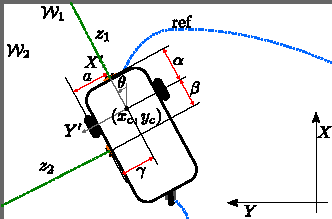
\includegraphics[scale=1.8]{figures/illustration_kalman.pdf}
\caption{Schematic overview of the robot moving in the world and measuring the distance to the walls. $(x_{\mathrm{c}},y_{\mathrm{c}})$ are the coordinates of the robot's center in the world coordinate system $XY$. The robot's orientation is determined by $\theta$, the angle between the $X$-axis and the robot's longitudinal axis $X'$. The dimensions $a$ and $\alpha,\beta,\gamma$ are to be measured for the state equations and output equations respectively.}
\label{fig:cartkalman}
\end{figure}

\newpage
\begin{enumerate}
  \item Model the system.
  \begin{enumerate}
    \item Write down the state equation. The input of the system can be chosen as $u = \begin{bmatrix}v\\ \omega\end{bmatrix}$, where $\omega$ [rad/s] denotes the rotational velocity of the robot around its center point, and $v$ [m/s] is the robot's forward translational velocity (i.e. along its longitudinal axis). Use a forward Euler method to discretize the system.
    \item Write down the measurement equation for the infrared sensors ($z_1$, $z_2$). Assume that a (straight) wall is characterized by $\mathcal{W} = \{(x,y) \,|\, px+qy=r\}$. The dimensions $\alpha$, $\beta$, $\gamma$ and $a$ can be measured on your platform if required.
  \end{enumerate}

  \item Design and implement an extended Kalman filter.
  \begin{enumerate}
    \item Two sources of noise are incorporated in the model. Measurement noise is added to the output equation and is assumed to have a normal distribution with zero mean and a diagonal covariance matrix $R$. Process noise is added to the state equation and is assumed to have a normal distribution with zero mean and a diagonal covariance matrix $Q$. What are potential sources of process noise?
    \item As you should have noticed, the system equations are nonlinear. Therefore an extended Kalman filter is used to estimate the states. This filter linearizes the state and measurement equations around the current estimated state. Write down the Jacobian of the state equation and measurement equation.
    \item Implement the steps of the extended Kalman filter on the Arduino. Apply an input velocity of choice to the system. Make sure that both infrared sensors still have a line of sight with their corresponding wall.
    Monitor the evolution of the estimation error covariance $\hat{P}_{k|k}$ and Kalman gain $L_k$ for different values of $\frac{Q}{R}$. Explain what happens when decreasing/increasing $\frac{Q}{R}$.
    \item Eliminate one of the two measurement equations. Apply an input velocity to the system and monitor the evolution of $\hat{P}_{k|k}$. Draw confidence ellipsoids in the XY-plane based on $\hat{P}_{k|k}$. How are they converging? Explain this.
  \end{enumerate}
  \item Design and implement a state feedback controller for following a position and orientation trajectory. This controller takes as input the tracking error
  \begin{equation}
  \hat{e} = \begin{bmatrix}
  x_{c,\text{ref}}-\hat{x}_c\\
  y_{c,\text{ref}}-\hat{y}_c\\
  \theta_{\text{ref}}-\hat{\theta}\\
  \end{bmatrix}
  \end{equation}
  As the system to be controlled is nonlinear and only design approaches for linear systems were addressed during the course, a heuristic control approach is proposed to design the state feedback controller. The control law is computed by first expressing the state error in the coordinate system $X'Y'$ attached to the cart (see Figure \ref{fig:cartkalman}).
  \begin{enumerate}
    \item Determine the rotation matrix that is required for the conversion of $(x,y,\theta)$, expressed in the world coordinate system $XY$, to $(x',y',\theta')$, expressed in the local coordinate system $X'Y'$. As this conversion depends on the orientation $\theta$ of the cart, use the estimate $\hat{\theta}_k$ to convert $\hat{e}_k$ to $\hat{e}'_k$.
    \item A static feedback matrix $K$ is proposed to compute $u$ from $\hat{e}'$ ($u = K \hat{e}'$) with the following structure:
    \begin{equation}
      K = \begin{bmatrix} k_x & 0 & 0 \\ 0 & k_y & k_\theta \end{bmatrix}\,
    \end{equation}
    Explain why this structure makes sense.
    \item Use a systematic approach to tune the values for $k_x$, $k_y$ and $k_\theta$. Illustrate the influence of changing these control parameters with relevant plots.
    \item Improve the tracking performance by adding an explicit feedforward signal to the system input: ${u=u_{FF}+K\hat{e}'}$. Illustrate the performance of the overall system by plotting tracking errors.
  \end{enumerate}
\end{enumerate}

\end{document}
